\documentclass{IEEEtran}
%% PACKAGES %%

\hbadness=99999

\usepackage{amsmath, amsfonts, amssymb, amsthm}
\usepackage{braket}
\usepackage{listings}
\usepackage{geometry}
\usepackage{xcolor}
\usepackage{textcomp}
\usepackage{graphicx}
\usepackage{fancyhdr}
\usepackage{sourcecodepro}
\usepackage{multirow}

%%%%%%%%%%%%%%

\graphicspath{{./images}}

%% LISTINGS CONFIG %%

\definecolor{purple2}{RGB}{153,0,153} % there's actually no standard purple
\definecolor{green2}{RGB}{0,153,0} % a darker green

\lstset{
  language=MATLAB,                   % the language
  basicstyle=\normalsize\ttfamily,   % size of the fonts for the code
  frame = single,
  % Color settings to match IDLE style
  keywordstyle=\color{orange},       % core keywords
  keywordstyle={[2]\color{purple2}}, % built-ins
  stringstyle=\color{green2},%
  showstringspaces=false,
  commentstyle=\color{red},%
  upquote=true,                      % requires textcomp
  numbers=left,
  breaklines=true,
}

% Title Stuff
\title{\vspace{-3cm} FIR and IIR Filter Design}
\author{Chase A. Lotito, \textit{SIUC Undergraduate}}
\date{}

\begin{document}

\pagestyle{fancy}

% attempt to make nice header
\fancyhead{}
\fancyhead[CH]{\normalsize{LOTITO - SIUC - ECE355L Project 5}}

\maketitle % Makes the title

\section{Experimental Results}

\subsection{Task I: FIR Filter}

\begin{figure}[!ht] 
    \centering
    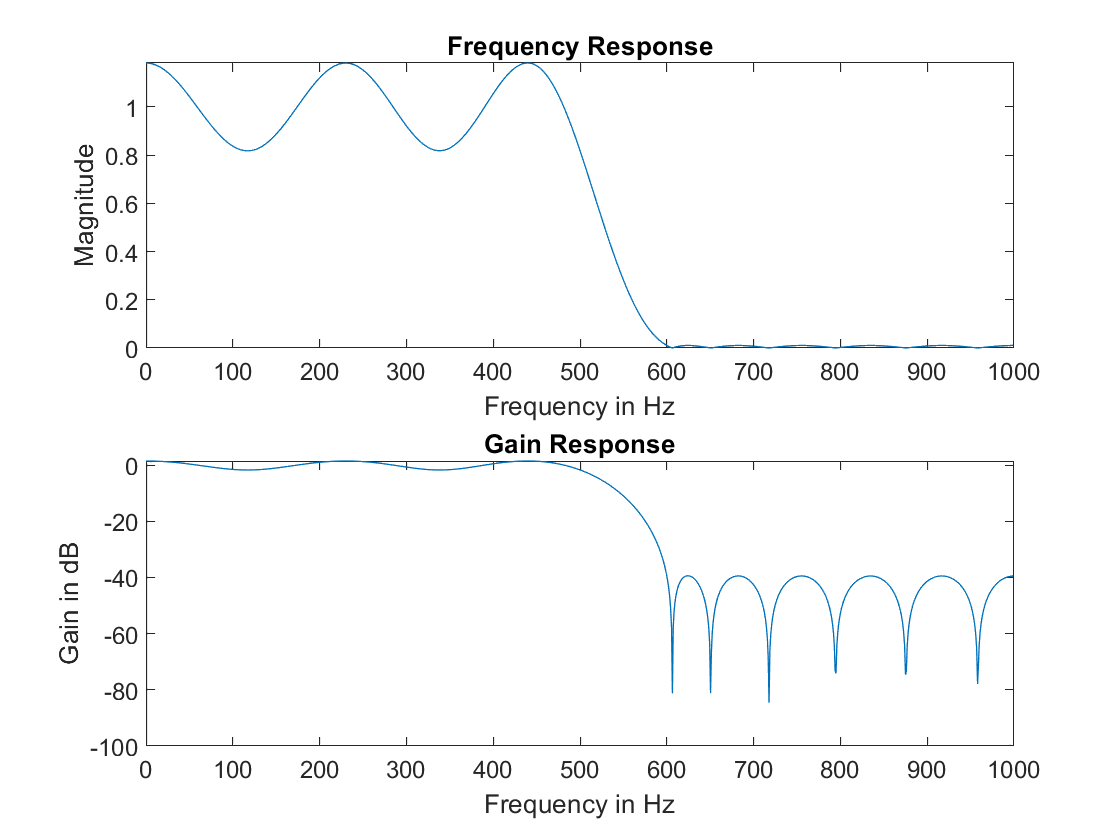
\includegraphics[width = 7cm]{task1.png}
    \caption{FIR low-pass filter.}
    \label{fig:task1}
\end{figure}

\subsection{Task II: Butterworth and Chebyshev IIR Filters}

\begin{figure}[!ht] 
    \centering
    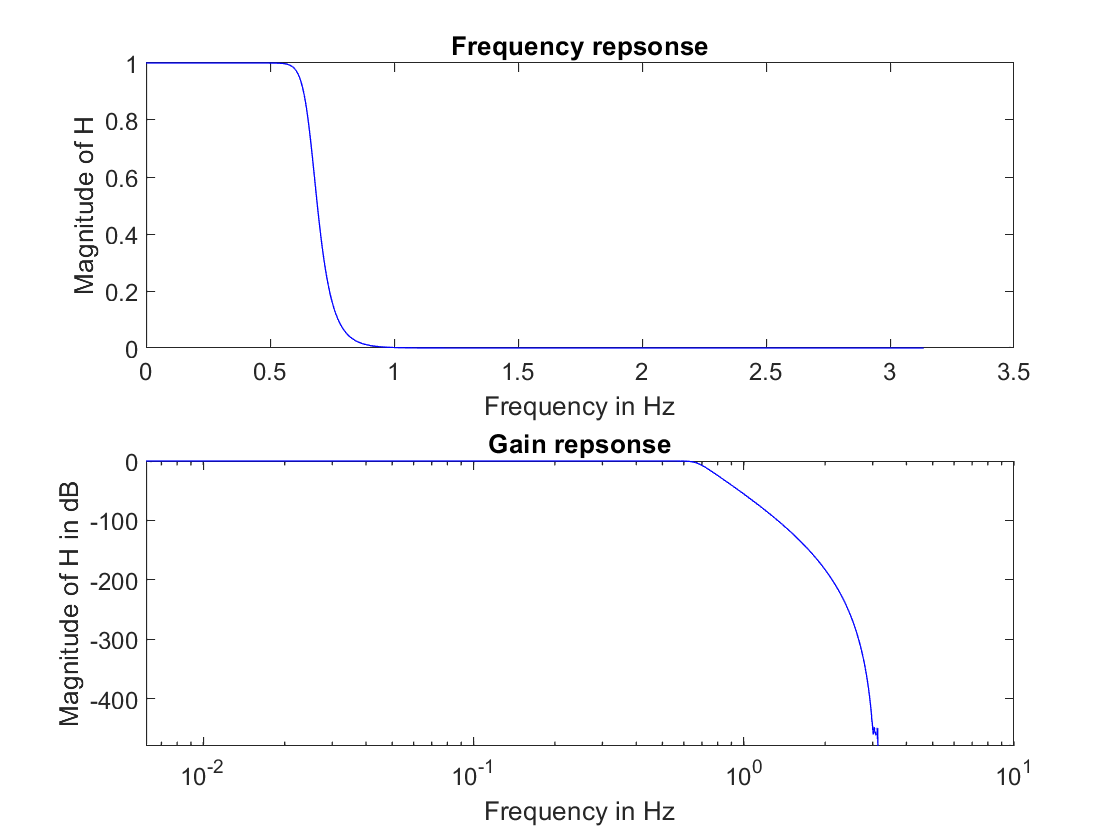
\includegraphics[width = 7cm]{butterworth.png}
    \caption{IIR Butterworth filter.}
    \label{fig:butterworth}
\end{figure}

\begin{figure}[!ht] 
    \centering
    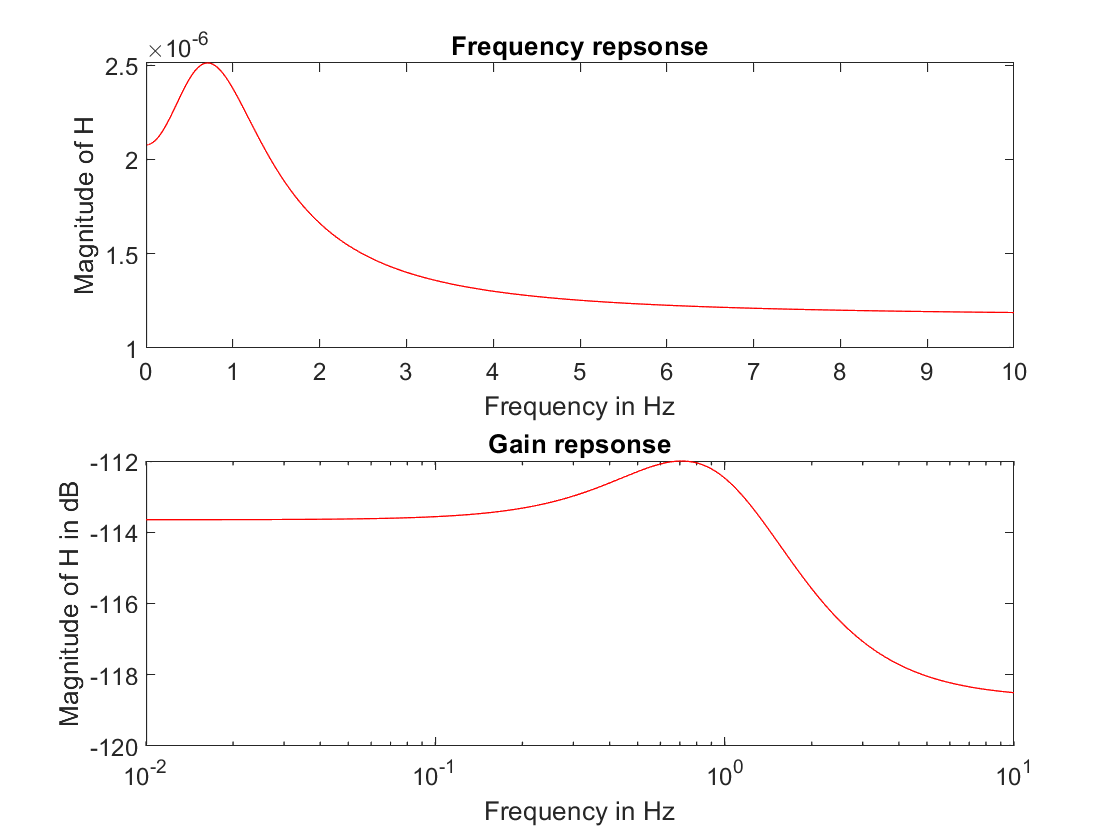
\includegraphics[width = 7cm]{chebyshev.png}
    \caption{IIR Chebyshev filter.}
    \label{fig:chebyshev}
\end{figure}

\section{Discussion}
% Please discuss your understanding of the digital filter design with considerations of public health, safety, and welfare, as well as global, cultural, social, environmental, and economic factors. (This discussion could be in general and should not be limited to the tasks of IIR and FIR filters design).

Butterworth filters have smooth and flat passbands with slow roll-off in the stopband, and Chebyshev filters have ripples in their pass and stopbands but quicker rolloff \cite{textbook}. For the Chebyshev filter, we implemented a Type I, which has the ripples in the passband. Both filters here are implemented as low-pass filters, which pass low-frequency signals and stop high-frequency signals.

Essentially, Butterworth filters are critical for applications that need smooth frequency response, and Chebyshev filters are critical for applications that need a sharp cutoff, or strongly restricted stopband.

Butterworth filters are best in applications like audio processing, since for desired frequencies, there won't be moments of unnecessary attenuation. Culturally and socially, robust audio-systems allow for enhanced communication and entertainment---these systems fundamentally produce and propogate modern culture. Also, in applications like air-traffic control, it is necessary that audio-based communications retain as much fidelity as possible to ensure clear lines of information can be sent, which is paramount for the safety of pilots and passengers. 

Chebyshev filters are more suited for high-frequency, radar, and other sensing applications. The steeper roll-off allows cleaner distinctions between the desired low-frequencies and undesirable high-frequencies. This can be critical in noise-reduction for medical applications (i.e. pacemakers), and for public saftey in meterological radar systems.

% TODO: put references
\bibliographystyle{IEEEtran}
\bibliography{project5Bib.bib}

\end{document}
